% =============================================================================
% PART B - MODULE 33: DISPUTE RESOLUTION & EXPERT ARBITRATION (UC-33.01 - 33.10)
% In Charge: Vo Nhut Tin (CE180619)
% =============================================================================

\newpage
\subsection{Module 33: Dispute Resolution \& Expert Arbitration}

The Dispute Resolution \& Expert Arbitration module provides a structured two-tier conflict resolution framework protecting escrow funds whenever Client and Freelancer disagree on deliverable quality, scope changes, or delays: \textbf{Step 1 (Mutual Resolution within 48 hours)} and \textbf{Step 2 (Escalated Binding Arbitration by a Domain Expert)}.

% -----------------------------------------------------------------------------
\subsubsection{M33.01 -- Open Formal Dispute (UC-33.01)}

\begin{itemize}[leftmargin=1.5em,itemsep=2pt]
  \item \textbf{Screen Name \& Route Path:} Resolution Center Open Dispute Drawer -- \texttt{/[role]/\allowbreak{}contracts/\allowbreak{}[slug]/\allowbreak{}milestones/\allowbreak{}[milestoneId]}.
  \item \textbf{Target Actor:} Client, Freelancer.
  \item \Needspace{6\baselineskip}\textbf{Before You Begin:} Milestone is funded (\texttt{FUNDED}), not yet completed, and has no open active dispute.
\end{itemize}
\begin{figure}[H]\centering
  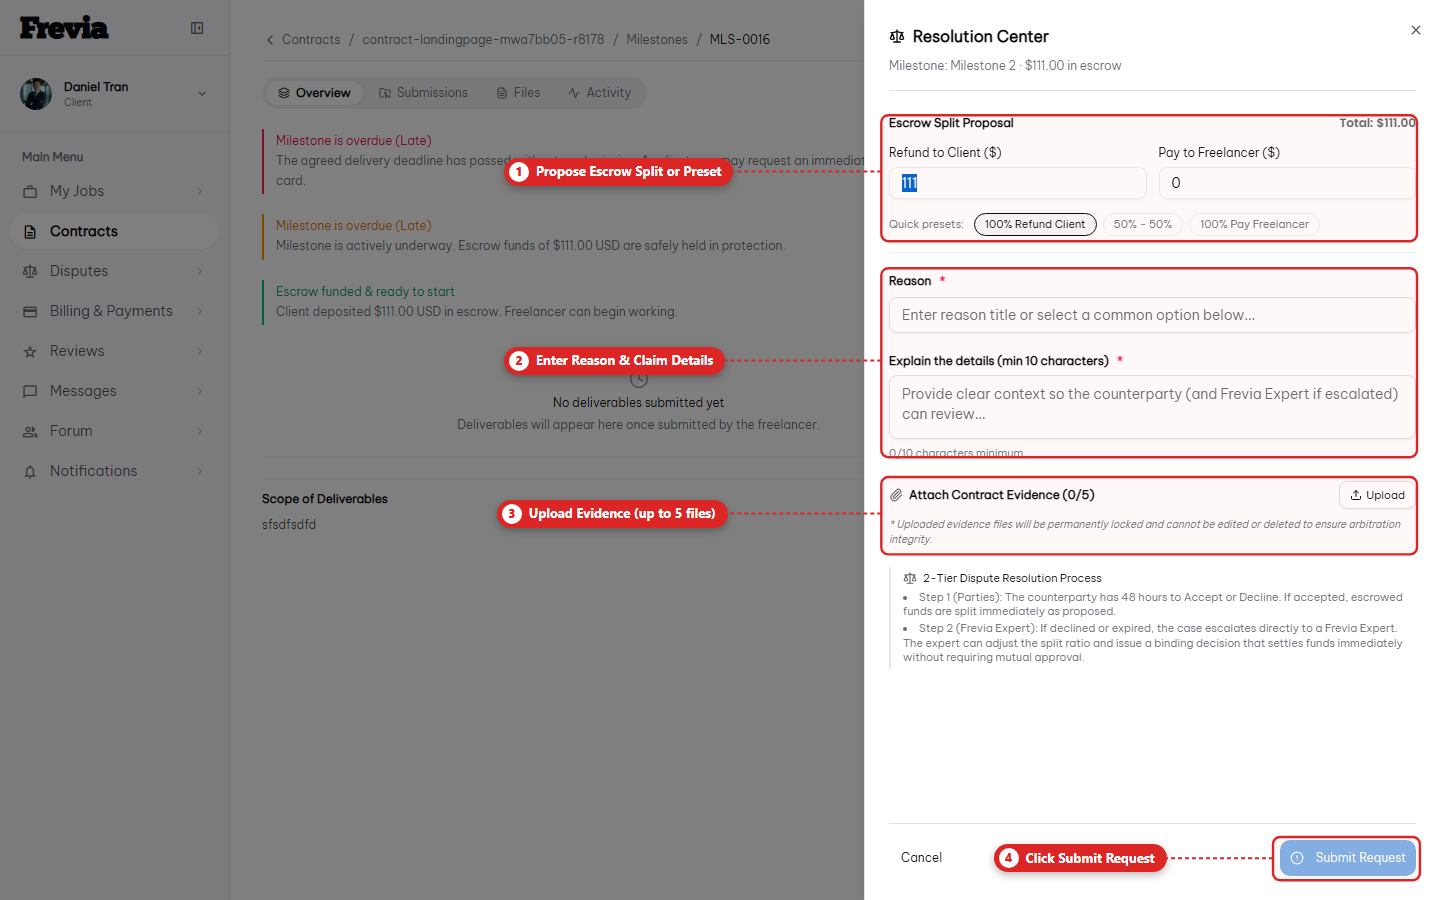
\includegraphics[width=0.90\textwidth]{images/disputes/m33_01_open_dispute_guide.png}
  \caption{Resolution Center drawer for proposing escrow split and uploading evidence}
  \label{fig:m33_01_open_dispute}
\end{figure}
\Needspace{6\baselineskip}\paragraph{Step-by-Step User Guide:}
\begin{enumerate}[leftmargin=1.8em,itemsep=3pt]
  \item \rbadge{1} \textbf{Propose Escrow Split or Preset:} Specify \textit{Refund to Client (\$)} and \textit{Pay to Freelancer (\$)} using custom amounts or quick presets (\textit{100\% Refund Client}, \textit{50\% -- 50\%}, \textit{100\% Pay Freelancer}).
  \item \rbadge{2} \textbf{Enter Reason \& Claim Details:} Select or type a clear \textit{Reason *} title and write a detailed narrative explanation (minimum 10 characters).
  \item \rbadge{3} \textbf{Upload Evidence (up to 5 files):} Click \textbf{Upload} under \textit{Attach Contract Evidence} to attach locked supporting screenshots, logs, or documents.
  \item \rbadge{4} \textbf{Click Submit Request:} Click \textbf{Submit Request} to freeze milestone escrow and notify your counterparty.
\end{enumerate}
\Needspace{6\baselineskip}\paragraph{After You Submit (Result \& Troubleshooting):}
\begin{itemize}[leftmargin=1.5em,itemsep=2pt]
  \item \textbf{What Happens Next:} Case status initializes at \texttt{WAITING\_RESPONSE}, milestone escrow locks from release/refund, and a 48-hour counterparty response timer begins.
  \item \textbf{Troubleshooting \& Common Messages:} Uploaded evidence files are permanently locked for arbitration integrity; exceeding 5 files or mismatched split sums triggers HTTP 400/422.
\end{itemize}

% -----------------------------------------------------------------------------
\newpage
\subsubsection{M33.02 -- View Disputes List (UC-33.02)}

\begin{itemize}[leftmargin=1.5em,itemsep=2pt]
  \item \textbf{Screen Name \& Route Path:} Disputes \& Arbitration Center -- \texttt{/client/\allowbreak{}disputes} or \texttt{/freelancer/\allowbreak{}disputes}.
  \item \textbf{Target Actor:} Client, Freelancer.
  \item \Needspace{6\baselineskip}\textbf{Before You Begin:} Signed in as Client or Freelancer.
\end{itemize}
\begin{figure}[H]\centering
  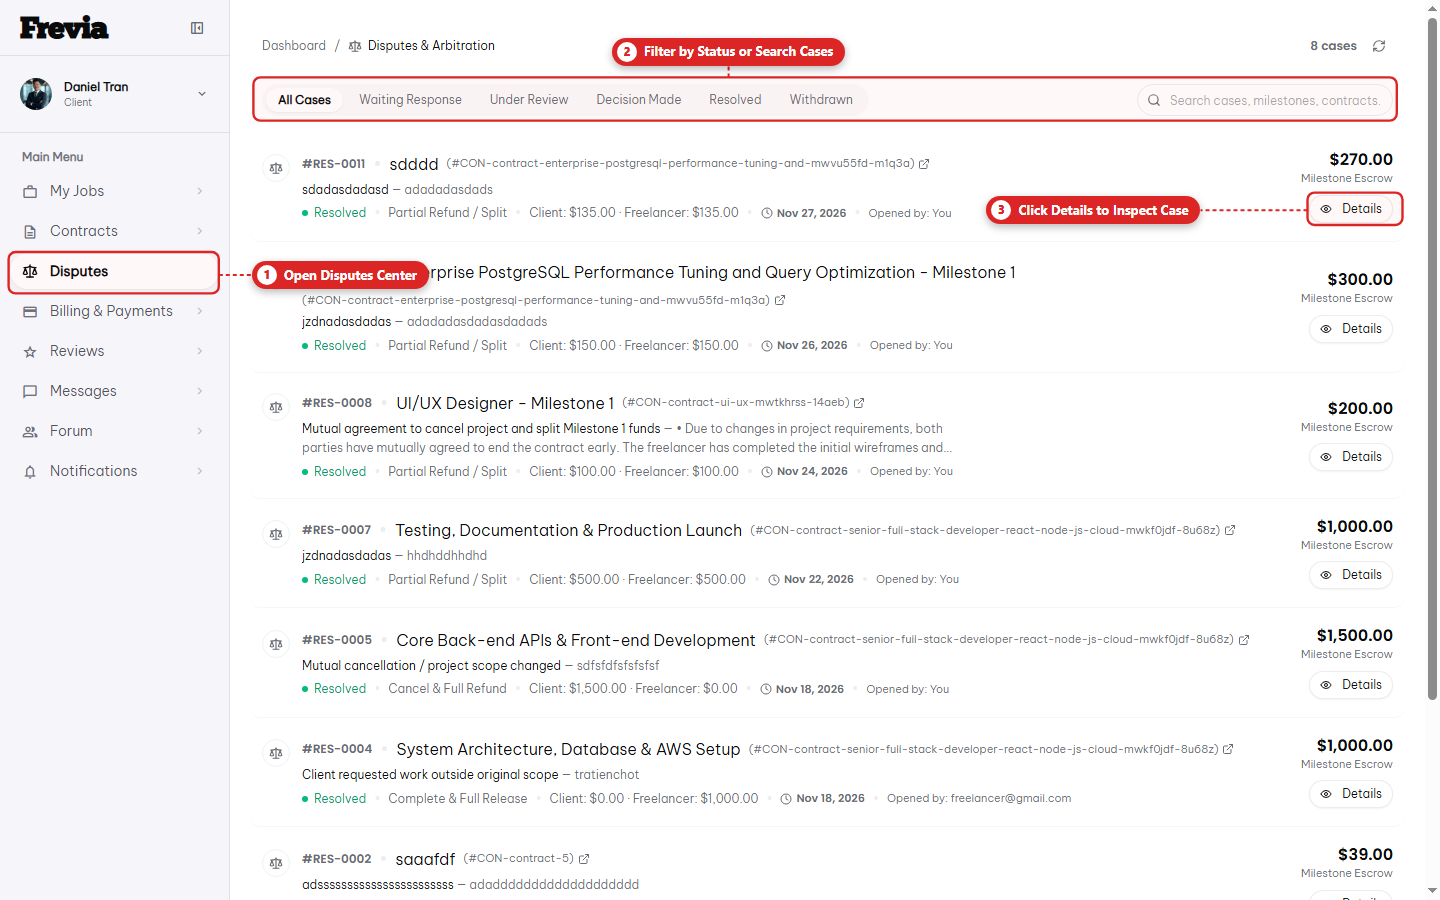
\includegraphics[width=0.90\textwidth]{images/disputes/m33_02_view_dispute_list_guide.png}
  \caption{Disputes \& Arbitration queue displaying filter tabs, split outcomes, and details trigger}
  \label{fig:m33_02_view_dispute_list}
\end{figure}
\Needspace{6\baselineskip}\paragraph{Step-by-Step User Guide:}
\begin{enumerate}[leftmargin=1.8em,itemsep=3pt]
  \item \rbadge{1} \textbf{Open Disputes Center:} Click \textbf{Disputes} in the left sidebar navigation.
  \item \rbadge{2} \textbf{Filter by Status or Search Cases:} Filter by \textbf{All Cases}, \textbf{Waiting Response}, \textbf{Under Review}, \textbf{Decision Made}, \textbf{Resolved}, or \textbf{Withdrawn}, or search by case number/title.
  \item \rbadge{3} \textbf{Click Details to Inspect Case:} Click \textbf{Details} on any case card (\texttt{\#RES-0011}, etc.) to open its arbitration timeline drawer.
\end{enumerate}
\Needspace{6\baselineskip}\paragraph{After You Submit (Result \& Troubleshooting):}
\begin{itemize}[leftmargin=1.5em,itemsep=2pt]
  \item \textbf{What Happens Next:} All disputes where you are initiator or respondent display with locked escrow amounts and resolution summaries.
  \item \textbf{Troubleshooting \& Common Messages:} Users without open or historical cases see an empty resolution center summary.
\end{itemize}

% -----------------------------------------------------------------------------
\newpage
\subsubsection{M33.03 -- View Dispute Case Details (UC-33.03)}

\begin{itemize}[leftmargin=1.5em,itemsep=2pt]
  \item \textbf{Screen Name \& Route Path:} Resolution Detail Drawer -- \texttt{/[role]/\allowbreak{}disputes}.
  \item \textbf{Target Actor:} Client, Freelancer (Case Participants).
  \item \Needspace{6\baselineskip}\textbf{Before You Begin:} Click \textbf{Details} on any dispute case entry.
\end{itemize}
\begin{figure}[H]\centering
  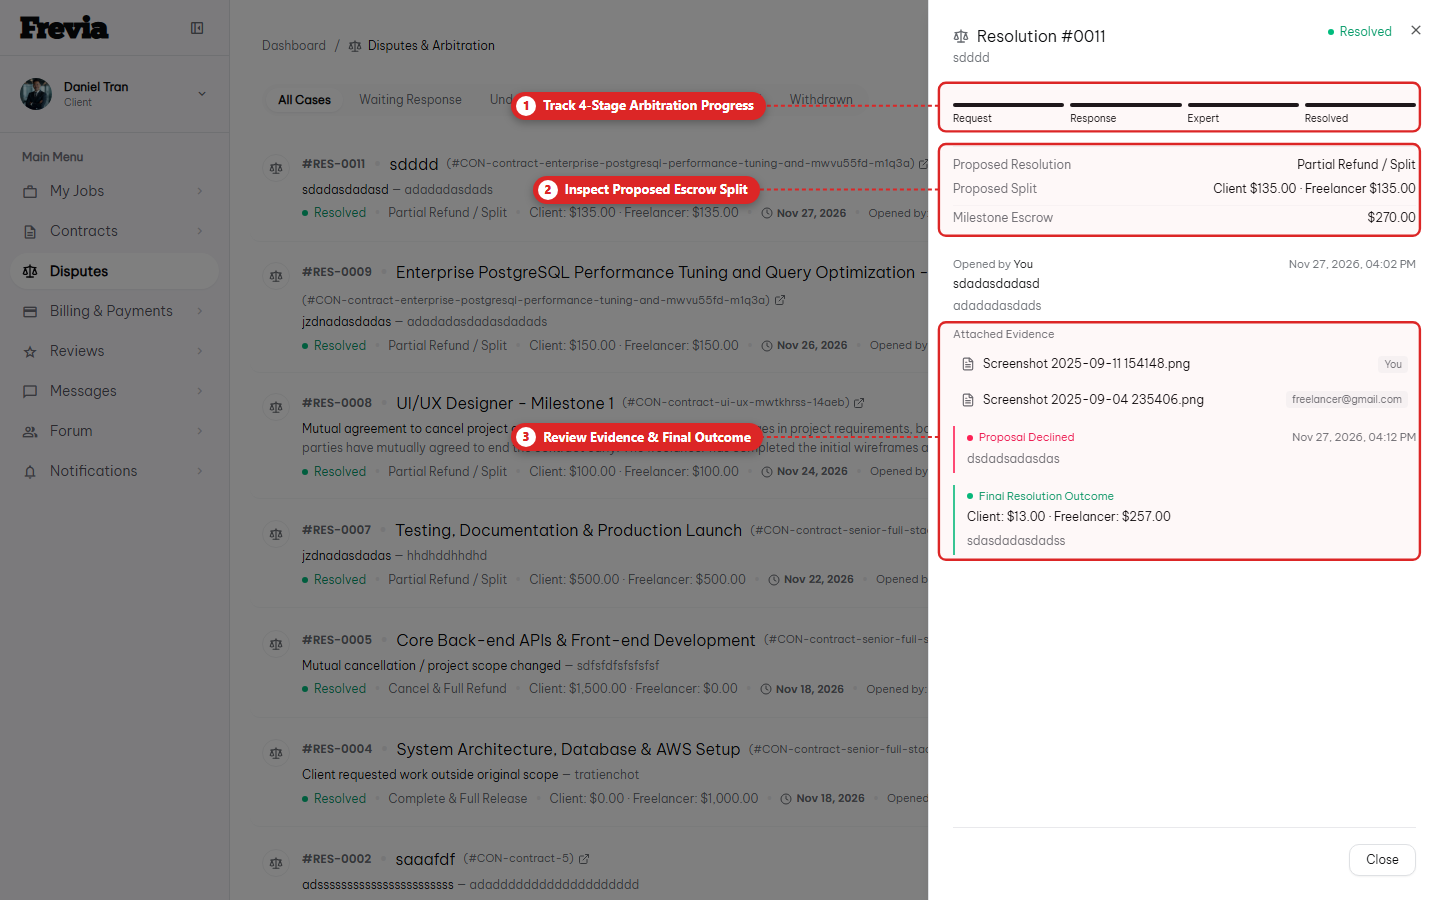
\includegraphics[width=0.90\textwidth]{images/disputes/m33_03_view_dispute_detail_guide.png}
  \caption{Resolution detail drawer showing 4-stage timeline, attached evidence, and final ruling}
  \label{fig:m33_03_view_dispute_detail}
\end{figure}
\Needspace{6\baselineskip}\paragraph{Step-by-Step User Guide:}
\begin{enumerate}[leftmargin=1.8em,itemsep=3pt]
  \item \rbadge{1} \textbf{Track 4-Stage Arbitration Progress:} Inspect the horizontal stepper across \textit{Request}, \textit{Response}, \textit{Expert}, and \textit{Resolved}.
  \item \rbadge{2} \textbf{Inspect Proposed Escrow Split:} Review the requested split amounts and total frozen milestone escrow balance.
  \item \rbadge{3} \textbf{Review Evidence \& Final Outcome:} Download attached evidence files from both sides, check any counterparty rebuttal notes, and read the \textit{Final Resolution Outcome}.
\end{enumerate}
\Needspace{6\baselineskip}\paragraph{After You Submit (Result \& Troubleshooting):}
\begin{itemize}[leftmargin=1.5em,itemsep=2pt]
  \item \textbf{What Happens Next:} Complete transparent case records and settlement transfers remain accessible for audit.
  \item \textbf{Troubleshooting \& Common Messages:} Non-participants requesting another party's dispute ID are rejected with HTTP 403 Forbidden.
\end{itemize}

% -----------------------------------------------------------------------------
\newpage
\subsubsection{M33.04 -- View Dispute by Milestone (UC-33.04)}

\begin{itemize}[leftmargin=1.5em,itemsep=2pt]
  \item \textbf{Screen Name \& Route Path:} Milestone Detail Dispute Lock View -- \texttt{/[role]/\allowbreak{}contracts/\allowbreak{}[slug]/\allowbreak{}milestones/\allowbreak{}[milestoneId]}.
  \item \textbf{Target Actor:} Client, Freelancer.
  \item \Needspace{6\baselineskip}\textbf{Before You Begin:} Open a milestone workspace linked to an active or resolved dispute.
\end{itemize}
\begin{figure}[H]\centering
  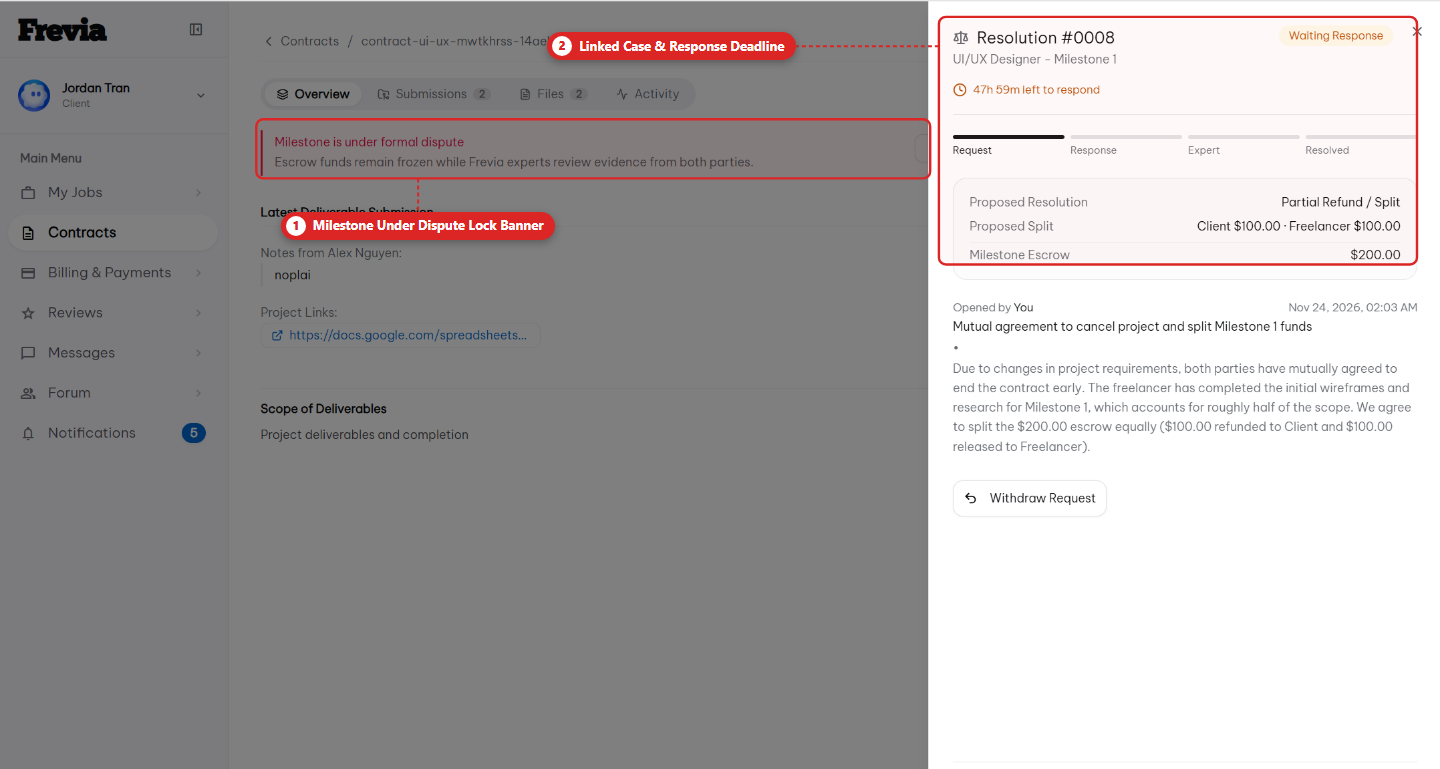
\includegraphics[width=0.90\textwidth]{images/disputes/m33_04_view_dispute_by_milestone_guide.png}
  \caption{Contextual dispute lock banner on milestone workspace synced via \texttt{GET /api/disputes/milestone/:milestoneId}}
  \label{fig:m33_04_view_dispute_by_milestone}
\end{figure}
\Needspace{6\baselineskip}\paragraph{Step-by-Step User Guide:}
\begin{enumerate}[leftmargin=1.8em,itemsep=3pt]
  \item \rbadge{1} \textbf{Milestone Under Dispute Lock Banner:} Observe the prominent alert banner explaining that escrow funds remain frozen while arbitration proceeds and standard submission/approval controls are locked.
  \item \rbadge{2} \textbf{Linked Case \& Response Deadline:} Open the contextual resolution drawer directly from the milestone view to monitor active split terms and the 48-hour countdown timer.
\end{enumerate}
\Needspace{6\baselineskip}\paragraph{After You Submit (Result \& Troubleshooting):}
\begin{itemize}[leftmargin=1.5em,itemsep=2pt]
  \item \textbf{What Happens Next:} Unilateral milestone approvals, modifications, or escrow releases stay strictly blocked until arbitration resolves or the claim is withdrawn.
  \item \textbf{Troubleshooting \& Common Messages:} Milestones with no associated dispute render normal workflow controls seamlessly.
\end{itemize}

% -----------------------------------------------------------------------------
\newpage
\subsubsection{M33.05 -- Respond to Dispute Proposal (UC-33.05)}

\begin{itemize}[leftmargin=1.5em,itemsep=2pt]
  \item \textbf{Screen Name \& Route Path:} Resolution Drawer (Respondent Action) -- \texttt{/[role]/\allowbreak{}contracts/\allowbreak{}[slug]/\allowbreak{}milestones/\allowbreak{}[milestoneId]} or \texttt{/[role]/\allowbreak{}disputes}.
  \item \textbf{Target Actor:} Client or Freelancer (Designated Respondent).
  \item \Needspace{6\baselineskip}\textbf{Before You Begin:} Counterparty opened a dispute in \texttt{WAITING\_RESPONSE} state within the 48-hour response window.
\end{itemize}
\begin{figure}[H]\centering
  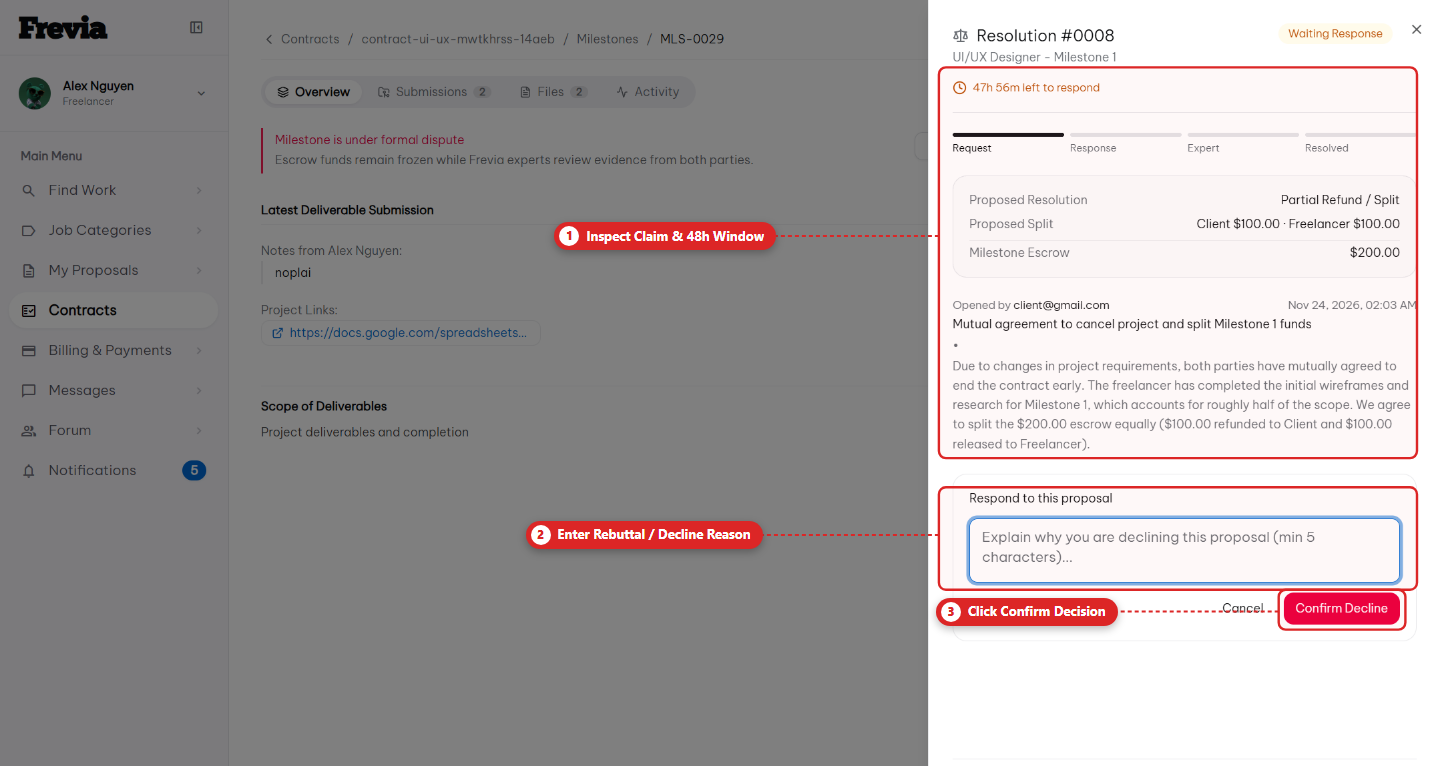
\includegraphics[width=0.90\textwidth]{images/disputes/m33_05_respond_to_dispute_guide.png}
  \caption{Respondent reviewing the claim and submitting an acceptance or reasoned decline}
  \label{fig:m33_05_respond_to_dispute}
\end{figure}
\Needspace{6\baselineskip}\paragraph{Step-by-Step User Guide:}
\begin{enumerate}[leftmargin=1.8em,itemsep=3pt]
  \item \rbadge{1} \textbf{Inspect Claim \& 48h Window:} Review the remaining response timer, proposed split amounts, and initiator's narrative.
  \item \rbadge{2} \textbf{Enter Rebuttal / Decline Reason:} Choose \textbf{Accept Proposal} to settle immediately, or click \textbf{Decline} and enter a detailed rebuttal (minimum 5 characters) with optional counter-evidence.
  \item \rbadge{3} \textbf{Click Confirm Decision:} Click \textbf{Confirm Decline} (or confirm acceptance) to transmit your formal response.
\end{enumerate}
\Needspace{6\baselineskip}\paragraph{After You Submit (Result \& Troubleshooting):}
\begin{itemize}[leftmargin=1.5em,itemsep=2pt]
  \item \textbf{What Happens Next:} Accepting settles escrow immediately as proposed; declining unlocks Expert Escalation (\textbf{M33.07}).
  \item \textbf{Troubleshooting \& Common Messages:} If 48 hours elapse without response, the dispute becomes eligible for direct Expert escalation.
\end{itemize}

% -----------------------------------------------------------------------------
\newpage
\subsubsection{M33.06 -- Withdraw Dispute Request (UC-33.06)}

\begin{itemize}[leftmargin=1.5em,itemsep=2pt]
  \item \textbf{Screen Name \& Route Path:} Resolution Drawer (Initiator Action) -- \texttt{/[role]/\allowbreak{}disputes}.
  \item \textbf{Target Actor:} Client or Freelancer (Dispute Initiator).
  \item \Needspace{6\baselineskip}\textbf{Before You Begin:} You initiated the dispute and no binding Expert ruling has been issued yet.
\end{itemize}
\begin{figure}[H]\centering
  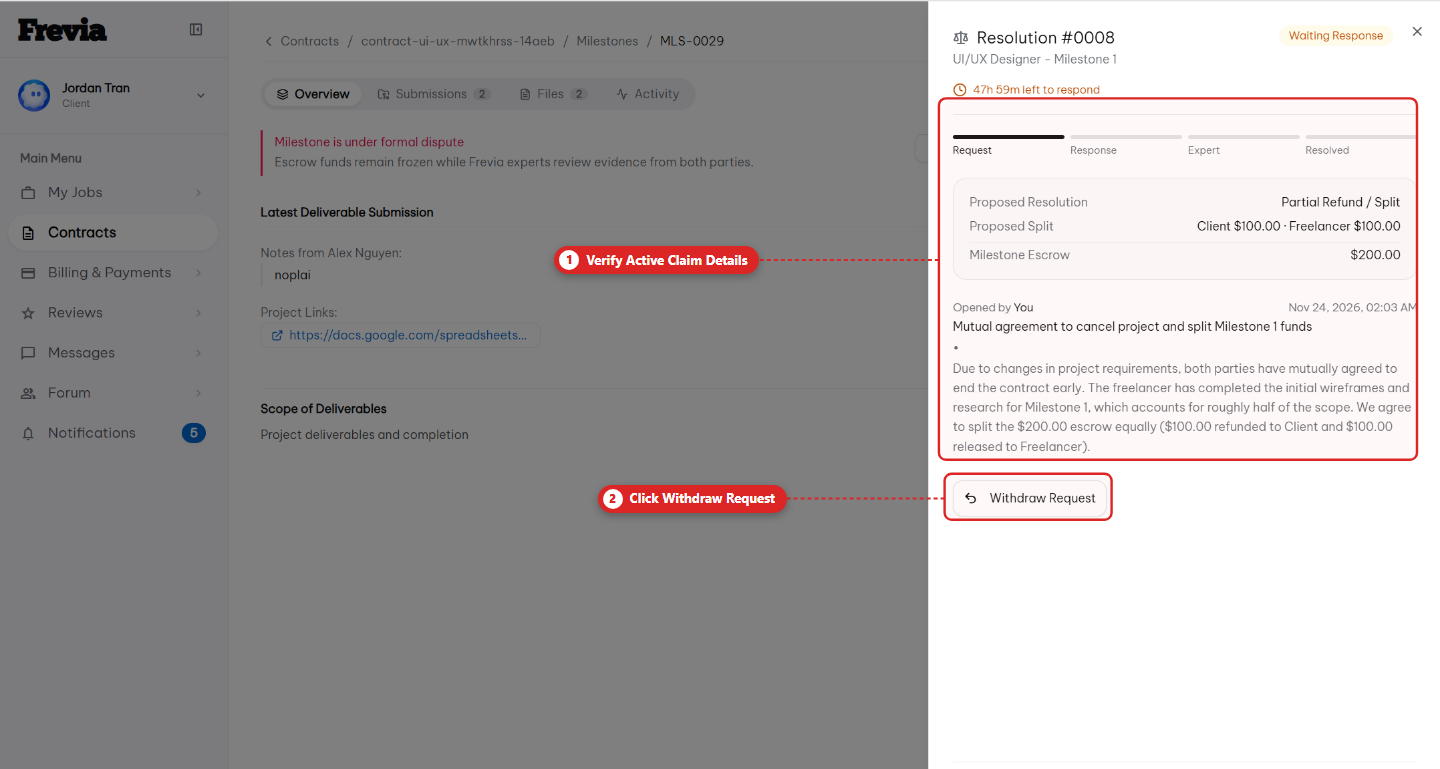
\includegraphics[width=0.90\textwidth]{images/disputes/m33_06_withdraw_dispute_guide.png}
  \caption{Initiator withdrawing an active dispute via Withdraw Request}
  \label{fig:m33_06_withdraw_dispute}
\end{figure}
\Needspace{6\baselineskip}\paragraph{Step-by-Step User Guide:}
\begin{enumerate}[leftmargin=1.8em,itemsep=3pt]
  \item \rbadge{1} \textbf{Verify Active Claim Details:} Open the active case drawer and review proposed amounts and status.
  \item \rbadge{2} \textbf{Click Withdraw Request:} Click \textbf{Withdraw Request} at the bottom of the drawer and confirm cancellation.
\end{enumerate}
\Needspace{6\baselineskip}\paragraph{After You Submit (Result \& Troubleshooting):}
\begin{itemize}[leftmargin=1.5em,itemsep=2pt]
  \item \textbf{What Happens Next:} Case status transitions to \texttt{WITHDRAWN}/\texttt{CANCELLED} and the milestone unlocks back to normal execution with escrow intact.
  \item \textbf{Troubleshooting \& Common Messages:} Only the original dispute initiator can withdraw a case; already-resolved cases cannot be withdrawn.
\end{itemize}

% -----------------------------------------------------------------------------
\newpage
\subsubsection{M33.07 -- Escalate Dispute to Expert (UC-33.07)}

\begin{itemize}[leftmargin=1.5em,itemsep=2pt]
  \item \textbf{Screen Name \& Route Path:} Resolution Drawer (Escalation Trigger) -- \texttt{/[role]/\allowbreak{}disputes}.
  \item \textbf{Target Actor:} Client, Freelancer.
  \item \Needspace{6\baselineskip}\textbf{Before You Begin:} Counterparty declined your Step 1 settlement proposal (\textit{Declined $\cdot$ Ready to Escalate}) or the 48-hour response deadline expired.
\end{itemize}
\begin{figure}[H]\centering
  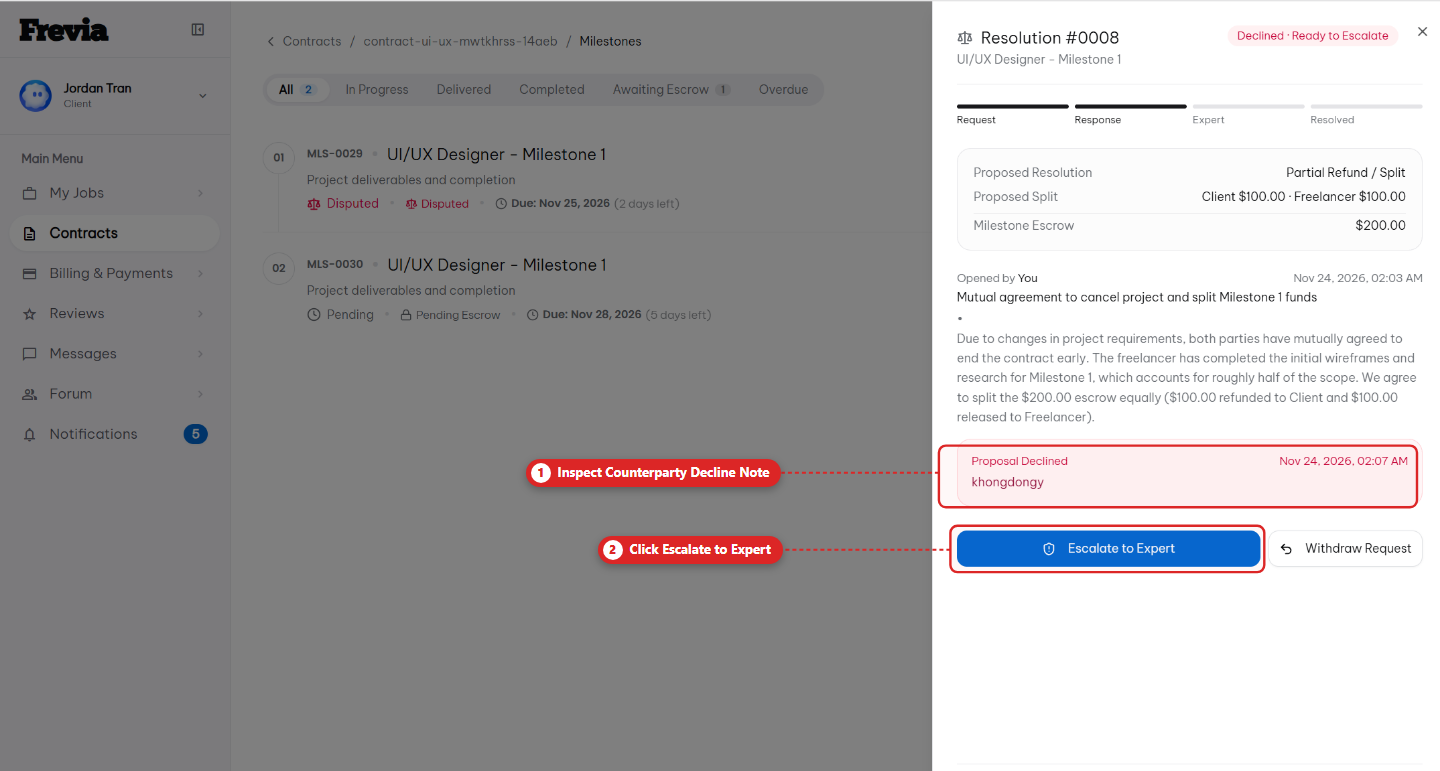
\includegraphics[width=0.90\textwidth]{images/disputes/m33_07_escalate_dispute_guide.png}
  \caption{Escalating a declined Step 1 dispute to a Frevia Expert arbitrator}
  \label{fig:m33_07_escalate_dispute}
\end{figure}
\Needspace{6\baselineskip}\paragraph{Step-by-Step User Guide:}
\begin{enumerate}[leftmargin=1.8em,itemsep=3pt]
  \item \rbadge{1} \textbf{Inspect Counterparty Decline Note:} Read the red \textit{Proposal Declined} box showing why the counterparty rejected the proposed split.
  \item \rbadge{2} \textbf{Click Escalate to Expert:} Click the blue \textbf{Escalate to Expert} button to advance the case into Step 2 Expert Arbitration.
\end{enumerate}
\Needspace{6\baselineskip}\paragraph{After You Submit (Result \& Troubleshooting):}
\begin{itemize}[leftmargin=1.5em,itemsep=2pt]
  \item \textbf{What Happens Next:} Status changes to \texttt{UNDER\_REVIEW} and the complete evidence dossier routes directly into the Expert Dispute Arbitration queue.
  \item \textbf{Troubleshooting \& Common Messages:} Escalation before counterparty decline or 48h timeout expiration is blocked with HTTP 422.
\end{itemize}

% -----------------------------------------------------------------------------
\newpage
\subsubsection{M33.08 -- View Expert Disputes Queue (UC-33.08)}

\begin{itemize}[leftmargin=1.5em,itemsep=2pt]
  \item \textbf{Screen Name \& Route Path:} Expert Dispute Arbitration Queue -- \texttt{/admin/\allowbreak{}disputes}.
  \item \textbf{Target Actor:} Expert (and Administrator with Dispute Permissions).
  \item \Needspace{6\baselineskip}\textbf{Before You Begin:} Signed in with \texttt{EXPERT} or authorized \texttt{ADMIN} portal credentials.
\end{itemize}
\begin{figure}[H]\centering
  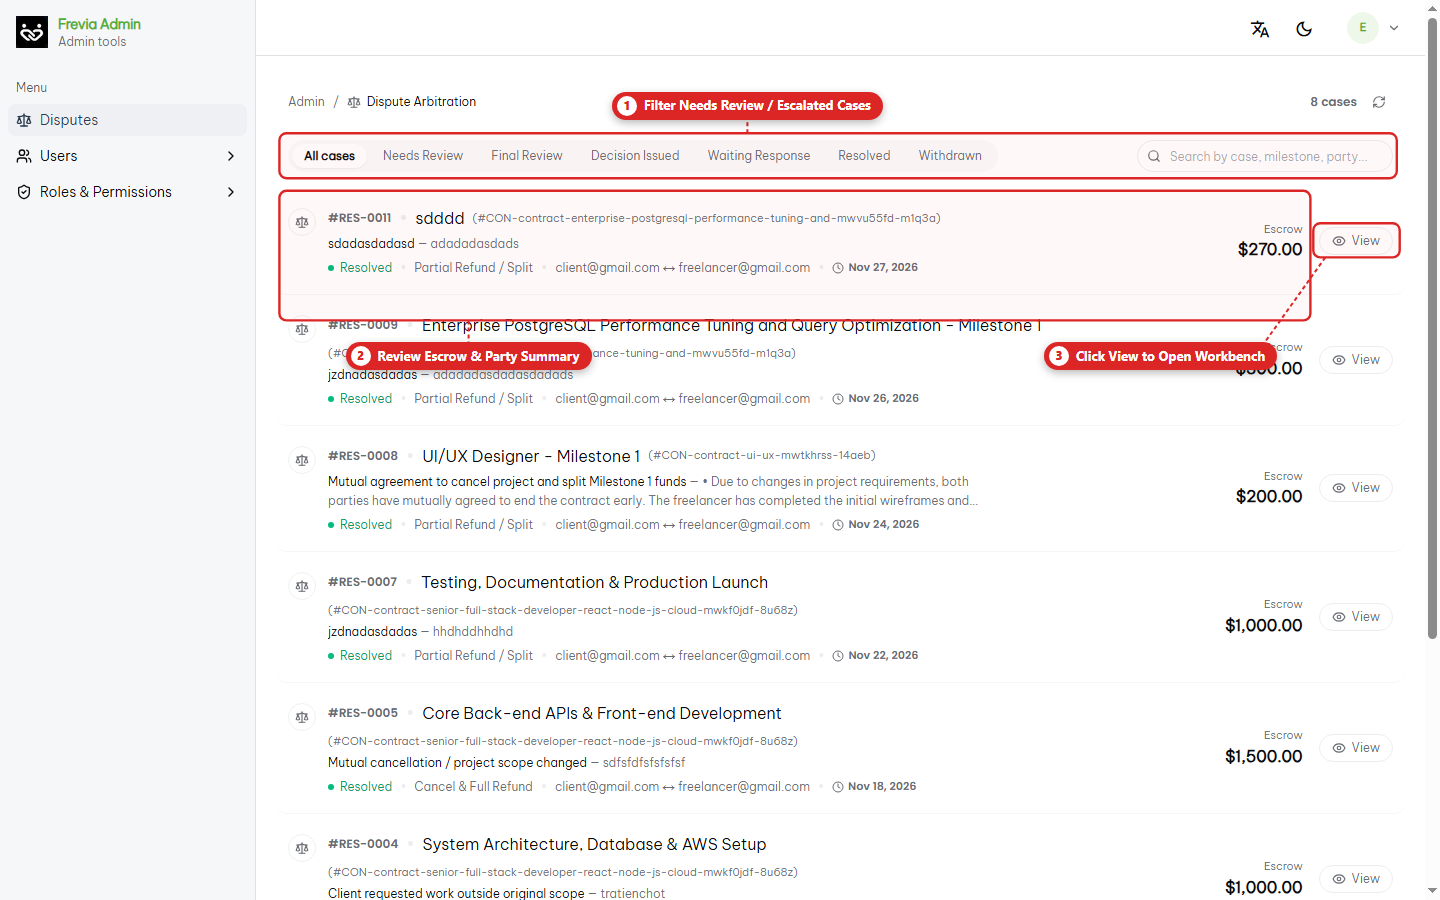
\includegraphics[width=0.90\textwidth]{images/disputes/m33_08_view_expert_dispute_list_guide.png}
  \caption{Expert Arbitration Console listing escalated and resolved dispute dossiers}
  \label{fig:m33_08_view_expert_dispute_list}
\end{figure}
\Needspace{6\baselineskip}\paragraph{Step-by-Step User Guide:}
\begin{enumerate}[leftmargin=1.8em,itemsep=3pt]
  \item \rbadge{1} \textbf{Filter Needs Review / Escalated Cases:} Filter across \textbf{All cases}, \textbf{Needs Review}, \textbf{Final Review}, \textbf{Decision Issued}, \textbf{Waiting Response}, \textbf{Resolved}, or \textbf{Withdrawn}.
  \item \rbadge{2} \textbf{Review Escrow \& Party Summary:} Scan dispute titles, Client/Freelancer emails, locked escrow balances, and escalation dates.
  \item \rbadge{3} \textbf{Click View to Open Workbench:} Click \textbf{View} beside a pending case to enter the full arbitration workbench.
\end{enumerate}
\Needspace{6\baselineskip}\paragraph{After You Submit (Result \& Troubleshooting):}
\begin{itemize}[leftmargin=1.5em,itemsep=2pt]
  \item \textbf{What Happens Next:} Escalated disputes requiring independent domain judgment load in priority order.
  \item \textbf{Troubleshooting \& Common Messages:} Standard Client/Freelancer accounts without RBAC dispute access are redirected away from \texttt{/admin/disputes}.
\end{itemize}

% -----------------------------------------------------------------------------
\newpage
\subsubsection{M33.09 -- View Expert Dispute Details (UC-33.09)}

\begin{itemize}[leftmargin=1.5em,itemsep=2pt]
  \item \textbf{Screen Name \& Route Path:} Expert Arbitration Dossier -- \texttt{/admin/\allowbreak{}disputes/\allowbreak{}[id]}.
  \item \textbf{Target Actor:} Expert / Administrator.
  \item \Needspace{6\baselineskip}\textbf{Before You Begin:} Click \textbf{View} on any case inside \texttt{/admin/disputes}.
\end{itemize}
\begin{figure}[H]\centering
  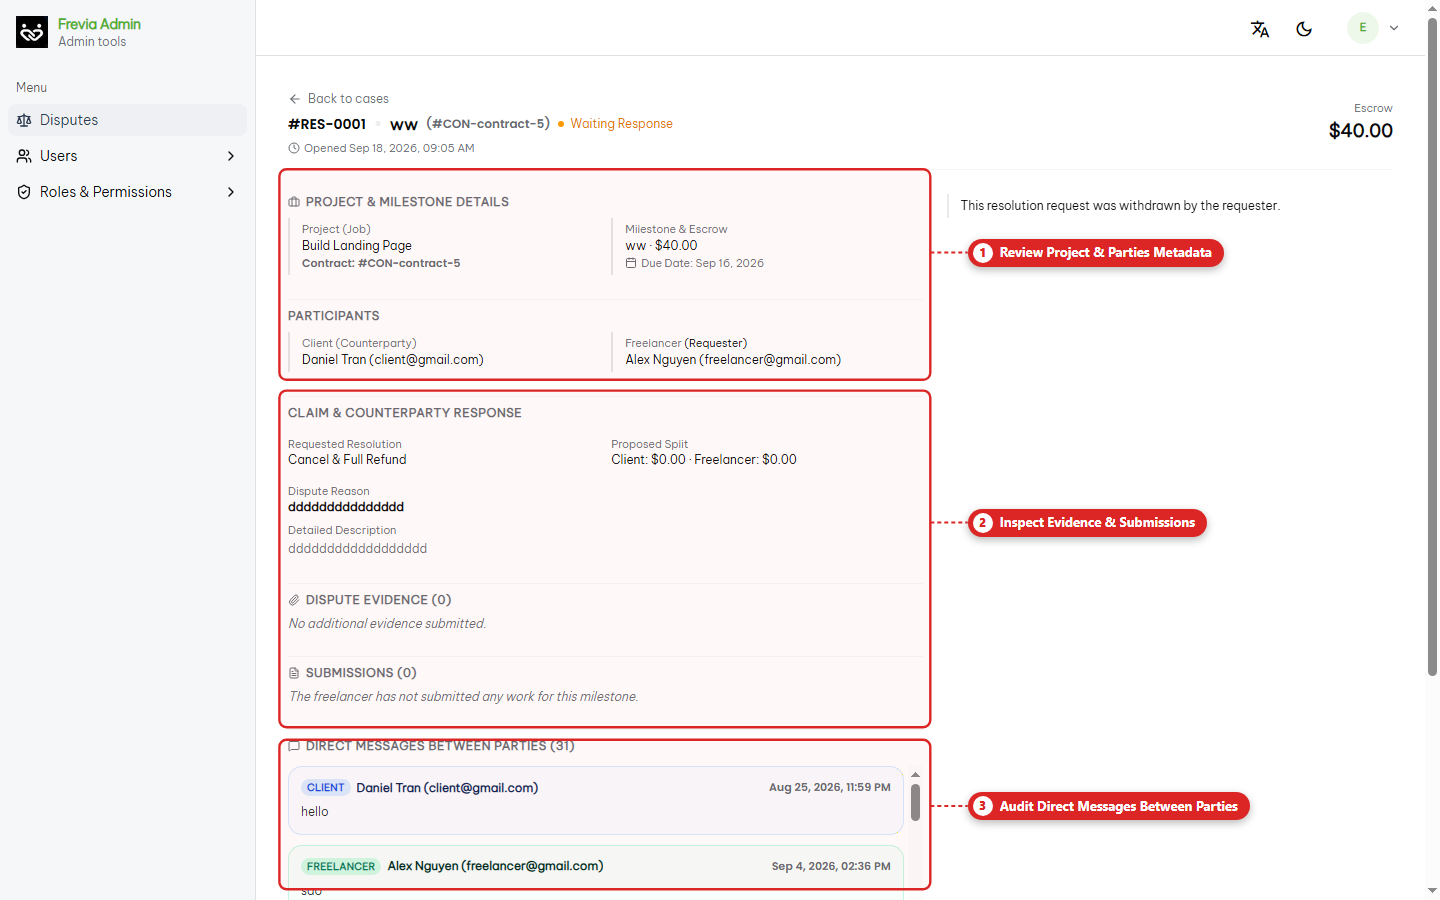
\includegraphics[width=0.90\textwidth]{images/disputes/m33_09_view_expert_dispute_detail_guide.png}
  \caption{Comprehensive Expert case file showing evidence, deliverables, and chat audit log}
  \label{fig:m33_09_view_expert_dispute_detail}
\end{figure}
\Needspace{6\baselineskip}\paragraph{Step-by-Step User Guide:}
\begin{enumerate}[leftmargin=1.8em,itemsep=3pt]
  \item \rbadge{1} \textbf{Review Project \& Parties Metadata:} Verify project title, milestone escrow value, deadline, and requester vs. counterparty details.
  \item \rbadge{2} \textbf{Inspect Evidence \& Submissions:} Examine claims, counterparty responses, attached dispute evidence, and submitted milestone deliverables.
  \item \rbadge{3} \textbf{Audit Direct Messages Between Parties:} Read the chronological message transcript between Client and Freelancer to verify agreed scope or delays.
\end{enumerate}
\Needspace{6\baselineskip}\paragraph{After You Submit (Result \& Troubleshooting):}
\begin{itemize}[leftmargin=1.5em,itemsep=2pt]
  \item \textbf{What Happens Next:} The Expert possesses all factual evidence necessary to issue an impartial, data-backed escrow ruling.
  \item \textbf{Troubleshooting \& Common Messages:} Withdrawn cases display an explicit banner noting the dispute was cancelled by the requester.
\end{itemize}

% -----------------------------------------------------------------------------
\newpage
\subsubsection[M33.10 -- Expert Make Dispute Decision (UC-33.10)]{M33.10 -- Issue Binding Arbitration Decision (UC-33.10)}

\begin{itemize}[leftmargin=1.5em,itemsep=2pt]
  \item \textbf{Screen Name \& Route Path:} Expert Arbitration Workbench -- \texttt{/admin/\allowbreak{}disputes/\allowbreak{}[id]}.
  \item \textbf{Target Actor:} Expert / Administrator.
  \item \Needspace{6\baselineskip}\textbf{Before You Begin:} Open an escalated case in \textit{Under Expert Review} state.
\end{itemize}
\begin{figure}[H]\centering
  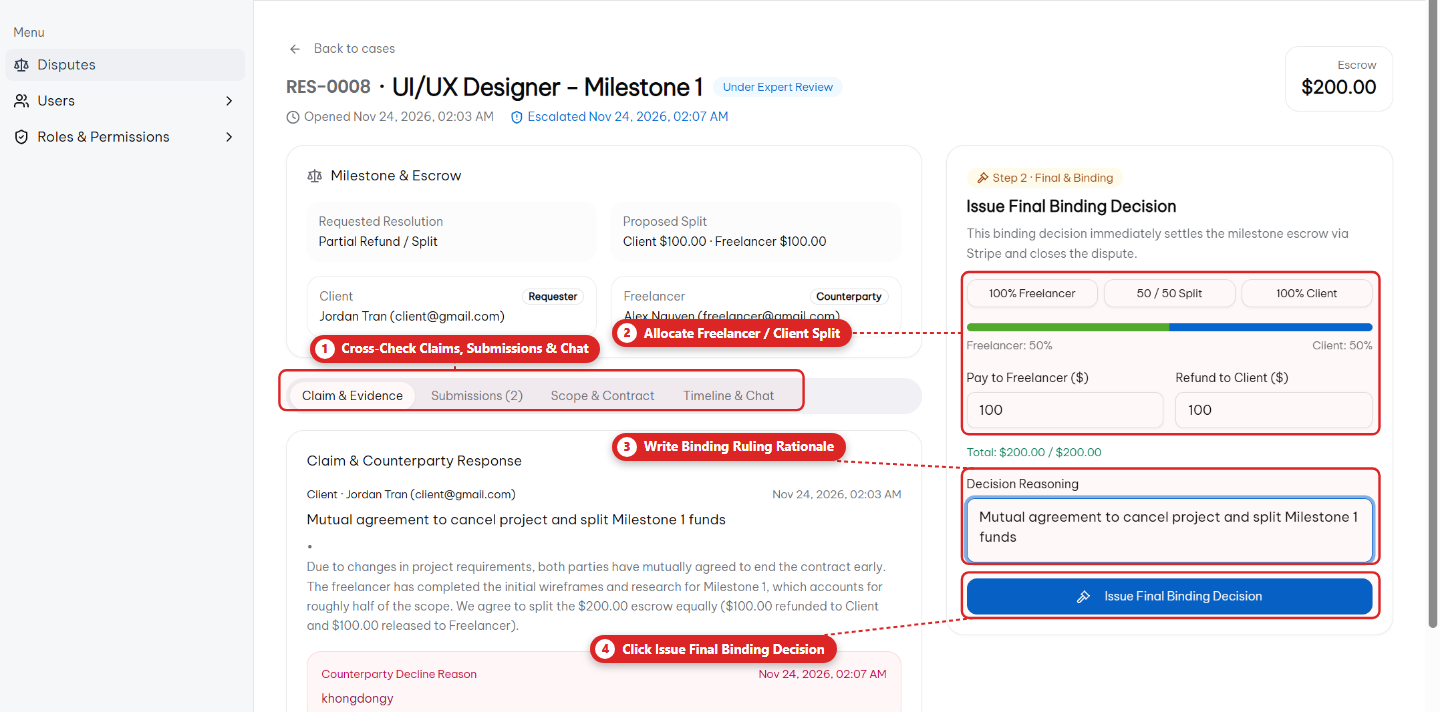
\includegraphics[width=0.90\textwidth]{images/disputes/m33_10_expert_decision_guide.png}
  \caption{Expert setting exact escrow split percentages and issuing a final binding decision}
  \label{fig:m33_10_expert_decision}
\end{figure}
\Needspace{6\baselineskip}\paragraph{Step-by-Step User Guide:}
\begin{enumerate}[leftmargin=1.8em,itemsep=3pt]
  \item \rbadge{1} \textbf{Cross-Check Claims, Submissions \& Chat:} Switch across \textbf{Claim \& Evidence}, \textbf{Submissions}, \textbf{Scope \& Contract}, and \textbf{Timeline \& Chat} tabs to validate facts.
  \item \rbadge{2} \textbf{Allocate Freelancer / Client Split:} Select a quick preset (\textbf{100\% Freelancer}, \textbf{50/50 Split}, \textbf{100\% Client}) or enter exact USD amounts summing to the full milestone escrow.
  \item \rbadge{3} \textbf{Write Binding Ruling Rationale:} Enter formal justification in \textit{Decision Reasoning} explaining why the split reflects evidence and contract terms.
  \item \rbadge{4} \textbf{Click Issue Final Binding Decision:} Click the blue \textbf{Issue Final Binding Decision} button to settle funds immediately via Stripe and close the case.
\end{enumerate}
\Needspace{6\baselineskip}\paragraph{After You Submit (Result \& Troubleshooting):}
\begin{itemize}[leftmargin=1.5em,itemsep=2pt]
  \item \textbf{What Happens Next:} Stripe automatically issues any Client refund and Freelancer Connect payout split, and the dispute status closes cleanly as \texttt{RESOLVED}.
  \item \textbf{Troubleshooting \& Common Messages:} The sum of Freelancer payout and Client refund must strictly equal the locked Milestone Escrow amount before submission succeeds.
\end{itemize}
